%% LyX 2.3.2 created this file.  For more info, see http://www.lyx.org/.
%% Do not edit unless you really know what you are doing.
\documentclass[english]{article}
\usepackage[T1]{fontenc}
\usepackage[latin9]{inputenc}
\usepackage{amsmath}
\usepackage{amssymb}
\usepackage{graphicx}

\makeatletter

%%%%%%%%%%%%%%%%%%%%%%%%%%%%%% LyX specific LaTeX commands.
%% A simple dot to overcome graphicx limitations
\newcommand{\lyxdot}{.}


\makeatother

\usepackage{babel}
\begin{document}
\title{GVINS}
\author{James Jackson}

\maketitle
\global\long\def\x{{\bf x}}%

\global\long\def\y{{\bf y}}%

\global\long\def\z{{\bf z}}%

\global\long\def\u{{\bf u}}%

\global\long\def\p{\mathbf{p}}%

\global\long\def\v{{\bf v}}%

\global\long\def\q{{\bf q}}%

\global\long\def\g{{\bf g}}%

\global\long\def\a{{\bf a}}%

\global\long\def\b{{\bf b}}%

\global\long\def\e{{\bf e}}%

\global\long\def\bt{\boldsymbol{\beta}}%

\global\long\def\al{\boldsymbol{\alpha}}%

\global\long\def\zt{\boldsymbol{\zeta}}%

\global\long\def\w{\boldsymbol{\omega}}%

\global\long\def\gm{\boldsymbol{\gamma}}%

\global\long\def\skew#1{\left\lfloor #1\right\rfloor _{\times}}%

\global\long\def\norm#1{\left\Vert #1\right\Vert }%


\section{IMU Preintegration}

We wish to marginalize IMU measurements in such a way that computing
a pose graph is efficient, but contains all the IMU information.

\begin{figure}[ht]
\centering{}\includegraphics[width=1\columnwidth]{/home/superjax/Documents/drawings/IMU_Preint_factor_graph\lyxdot svg}\caption{IMU Preintegration Factor Graph}
\label{fig:imu_factor_graph}
\end{figure}


\subsection{Derivation}

\begin{align*}
\x\left[i+1\right] & =F\left(\x\left[i\right],\u\left[i\right],\right)\\
\begin{bmatrix}\p_{j/I}^{I}\\
\v_{j/I}^{j}\\
\q_{I}^{j}
\end{bmatrix} & =\begin{bmatrix}\p_{i/I}^{I}+\p_{j/i}^{I}\\
R_{i}^{j}\left(\v_{i/I}^{i}+\v_{j/i}^{i}\right)\\
\q_{I}^{i}\otimes\q_{i}^{j}
\end{bmatrix}
\end{align*}

\[
\q_{I}^{b\left(t+\delta t\right)}=\q_{I}^{b\left(t\right)}\otimes\exp\left(\w_{b\left(t\right)/I}^{b\left(t\right)}\delta t\right)
\]

\[
\v_{j/i}^{j}=R_{i}^{j}\left(\int_{t}^{t+\delta t}R_{b\left(\tau\right)}^{i}\a_{b\left(\tau\right)/I}^{b\left(\tau\right)}\left(\tau\right)d\tau\right)
\]

\begin{align*}
\p_{j/i}^{I} & =\frac{1}{2}\g^{I}\delta t^{2}+\v_{i/I}^{I}\delta t+\int\int_{t}^{t+\delta t}R_{b\left(\tau\right)}^{I}\a_{b\left(\tau\right)/I}^{b\left(\tau\right)}\left(\tau\right)d\tau\\
 & =\frac{1}{2}\g^{I}\delta t^{2}+\v_{i/I}^{I}\delta t+R_{i}^{I}\int\int_{t}^{t+\delta t}R_{b\left(\tau\right)}^{i}\a_{b\left(\tau\right)/I}^{b\left(\tau\right)}\left(\tau\right)d\tau
\end{align*}

Let us isolate the parts of this derivation which is indepedent of
the initial state at the beginning of the interval, and call the remainder
$\y_{j/i}^{i}=\begin{bmatrix}\al & \gm & \bt\end{bmatrix}^{\top}$

\[
\begin{bmatrix}\p_{j/I}^{I}\\
\v_{j/I}^{j}\\
\q_{I}^{j}
\end{bmatrix}=\begin{bmatrix}\p_{i/I}^{I}+\frac{1}{2}\g^{I}\delta t^{2}+\v_{i/I}^{I}\delta t+R_{i}^{I}\al_{j/i}^{i}\\
R_{i}^{j}\left(\v_{i/I}^{i}+\bt_{j/i}^{i}\right)\\
\q_{I}^{b_{i}}\otimes\gm_{i}^{j}
\end{bmatrix}
\]

where

\[
\begin{bmatrix}\al_{j/i}^{i}\\
\bt_{j/i}^{i}\\
\gm_{i}^{j}
\end{bmatrix}=\begin{bmatrix}\int\int_{t}^{t+\delta t}R_{b\left(\tau\right)}^{I}\a_{b\left(\tau\right)/I}^{b\left(\tau\right)}\left(\tau\right)d\tau\\
\int_{t}^{t+\delta t}R_{b\left(\tau\right)}^{i}\a_{b\left(\tau\right)/I}^{b\left(\tau\right)}\left(\tau\right)d\tau\\
\int_{t}^{t+\delta t}\w_{b\left(\tau\right)/I}^{b\left(\tau\right)}d\tau
\end{bmatrix}
\]

We can write the continuous-time dynamics of $\y$ over the interval

\begin{align*}
\dot{\al}_{t/i}^{i} & =\bt_{t/i}^{i}\\
\dot{\bt}_{t/i}^{i} & =\left(R_{i}^{t}\right)^{\top}\a_{t/i}^{t}\\
\dot{\gm}_{i}^{t} & =\frac{1}{2}\left(\gm_{i}^{t}\otimes\begin{bmatrix}0\\
\w_{t/i}^{t}
\end{bmatrix}\right)
\end{align*}

and if we have an IMU measurement $\begin{bmatrix}\z_{a} & \z_{\omega}\end{bmatrix}^{\top}$
with constant bias $\begin{bmatrix}\b_{a} & \b_{\omega}\end{bmatrix}^{\top}$
and input noise $\eta_{\a},\eta_{\w}$

\begin{align*}
\dot{\al}_{t/i}^{i} & =\bt_{t/i}^{i}\\
\dot{\bt}_{t/i}^{i} & =\left(R_{i}^{t}\right)^{\top}\left(\z_{a}-\b_{a}+\eta_{\a}\right)\\
\dot{\gm}_{i}^{t} & =\frac{1}{2}\left(\gm_{i}^{t}\otimes\begin{bmatrix}0\\
\z_{\omega}-\b_{\omega}+\eta_{\w}
\end{bmatrix}\right).
\end{align*}


\subsection{Covariance Propagation}

If we assume that our acceleration measurement $\z_{a}$ is sampled
from some distribution $\mathcal{N}\left(\a+\b_{a},\Sigma_{a}\right)$
and that our angular rate measurement $\z_{\omega}$ is also sampled
from some distribution $\mathcal{N}\left(\w+\b_{\omega},\Sigma_{\omega}\right),$
then we can calculate the covariance of our preintegrated interval
using the error state.

\begin{align*}
\Sigma_{\y} & =E\left[\left(\y\boxminus\hat{\y}\right)\left(\y\boxminus\hat{\y}\right)^{\top}\right]\\
 & =E\left[\tilde{\y}\tilde{\y}^{\top}\right]
\end{align*}

where

\[
\y\boxminus\hat{\y}=\begin{bmatrix}\al-\hat{\al}\\
\bt-\hat{\bt}\\
\log_{q}\left(\hat{\gm}\otimes\gm^{-1}\right)
\end{bmatrix}.
\]
To propagate our covariance estimate over the interval, we will use
the dynamics of the error state. Before we derive these dynamics,
however, we must first define our error-state inputs for the gyro

\begin{align*}
\w_{b/i}^{i} & =\z_{\omega}-\b_{\omega}+\eta_{\omega}\\
\hat{\w}_{b/i}^{i} & =\z_{\omega}-\hat{\b}_{\omega}\\
\tilde{\w} & =\w-\hat{\w}\\
 & =\z_{\omega}-\b_{\omega}+\eta_{\omega}-\left(\z_{\omega}-\hat{\b}_{\omega}\right)\\
 & =-\tilde{\b}_{\omega}+\eta_{\omega}
\end{align*}
and likewise for the accelerometer

\begin{align*}
\a_{b/i}^{b} & =\z_{a}-\b_{a}+\eta_{a}\\
\hat{\a}_{\hat{b}/i}^{\hat{b}} & =\z_{a}-\hat{\b}_{a}\\
\tilde{\a} & =\a-\hat{\a}\\
 & =-\tilde{\b}_{a}+\eta_{a}.
\end{align*}

Using these definitions, the error-state $\tilde{\y}$ dynamics are
defined as follows: First let us consider $\al$, which turns out
to be pretty simple, because $\bt$ is already expressed in the origin
frame of the preintegration interval $i$

\[
\dot{\tilde{\al}}_{b/\hat{b}}^{i}=\bt_{b/i}^{i}-\bt_{\hat{b}/i}^{i}.
\]
The velocity-like term $\bt$ requires us to rotate our IMU measurements
into origin frame. To deal with this, we use the identity $R\left(\exp_{\q}\left(\boldsymbol{\delta}\right)\right)\approx I-\skew{\boldsymbol{\delta}}$
and drop all terms where error-quantities are multiplied together,
making the assumption that error-state quantities are small. This
is a reasonable assumption, because we will ultimately only use the
jacobian of these dynamics.

\begin{align*}
\dot{\tilde{\bt}}_{b/\hat{b}}^{i} & =\dot{\bt}_{b/i}^{i}-\dot{\hat{\bt}}_{b/i}^{b}\\
 & =\left(R_{i}^{b}\right)^{\top}\left(\a_{b/i}^{b}\right)-\left(R_{i}^{\hat{b}}\right)^{\top}\left(\hat{\a}_{\hat{b}/i}^{\hat{b}}\right)\\
 & =\left(\tilde{R}_{\hat{b}}^{b}\hat{R}_{i}^{\hat{b}}\right)^{\top}\left(\hat{\a}_{\hat{b}/i}^{\hat{b}}+\tilde{\a}_{\hat{b}/b}^{\hat{b}}\right)-\left(R_{i}^{\hat{b}}\right)^{\top}\left(\hat{\a}_{\hat{b}/i}^{\hat{b}}\right)\\
 & =\left(\hat{R}_{i}^{\hat{b}}\right)^{\top}R\left(\exp_{\q}\left(\tilde{\gm}_{\hat{b}}^{b}\right)\right)^{\top}\left(\hat{\a}_{\hat{b}/i}^{\hat{b}}+\tilde{\a}_{\hat{b}/b}^{\hat{b}}\right)-\left(R_{i}^{\hat{b}}\right)^{\top}\left(\hat{\a}_{\hat{b}/i}^{\hat{b}}\right)\\
 & \approx\left(\hat{R}_{i}^{\hat{b}}\right)^{\top}\left(I-\skew{\tilde{\gm}_{\hat{b}}^{b}}\right)^{\top}\left(\hat{\a}_{\hat{b}/i}^{\hat{b}}+\tilde{\a}_{\hat{b}/b}^{\hat{b}}\right)-\left(R_{i}^{\hat{b}}\right)^{\top}\left(\hat{\a}_{\hat{b}/i}^{\hat{b}}\right)\\
 & =\left(\hat{R}_{i}^{\hat{b}}\right)^{\top}\left(\hat{\a}_{\hat{b}/i}^{\hat{b}}+\tilde{\a}_{\hat{b}/b}^{\hat{b}}\right)+\left(\hat{R}_{i}^{\hat{b}}\right)^{\top}\skew{\tilde{\gm}_{\hat{b}}^{b}}\left(\hat{\a}_{\hat{b}/i}^{\hat{b}}+\tilde{\a}_{\hat{b}/b}^{\hat{b}}\right)-\left(R_{i}^{\hat{b}}\right)^{\top}\left(\hat{\a}_{\hat{b}/i}^{\hat{b}}\right)\\
 & =\left(\hat{R}_{i}^{\hat{b}}\right)^{\top}\left(\tilde{\a}_{\hat{b}/b}^{\hat{b}}\right)+\left(\hat{R}_{i}^{\hat{b}}\right)^{\top}\skew{\tilde{\gm}_{\hat{b}}^{b}}\left(\hat{\a}_{\hat{b}/i}^{\hat{b}}+\tilde{\a}_{\hat{b}/b}^{\hat{b}}\right)\\
 & \approx\left(\hat{R}_{i}^{\hat{b}}\right)^{\top}\left(\tilde{\a}_{\hat{b}/b}^{\hat{b}}\right)+\left(\hat{R}_{i}^{\hat{b}}\right)^{\top}\skew{\tilde{\gm}_{\hat{b}}^{b}}\hat{\a}_{\hat{b}/i}^{\hat{b}}\\
 & =\left(\hat{R}_{i}^{\hat{b}}\right)^{\top}\left(-\tilde{\b}_{a}+\eta_{\a}\right)+\left(\hat{R}_{i}^{\hat{b}}\right)^{\top}\skew{\tilde{\gm}_{\hat{b}}^{b}}\left(\z_{a}-\hat{\b}_{a}\right)\\
 & =-R\left(\gm_{i}^{\hat{b}}\right)^{\top}\left(\skew{\z_{a}-\hat{\b}_{a}}\tilde{\gm}_{\hat{b}}^{b}-\tilde{\b}_{a}+\eta_{\a}\right)
\end{align*}
Finally, we must also consider the attitude portion

\begin{align*}
\dot{\tilde{\gm}}_{b}^{\hat{b}} & =R\left(\exp_{\q}\left(\tilde{\gm}_{\hat{b}}^{b}\right)\right)\w_{b/i}^{b}-\hat{\w}_{\hat{b}/i}^{\hat{b}}\\
 & \approx\left(I-\skew{\tilde{\gm}_{\hat{b}}^{b}}\right)^{\top}\left(\hat{\w}_{\hat{b}/i}^{\hat{b}}+\tilde{\w}_{\hat{b}/b}^{\hat{b}}\right)-\hat{\w}_{\hat{b}/i}^{\hat{b}}\\
 & =\left(\hat{\w}_{\hat{b}/i}^{\hat{b}}+\tilde{\w}_{\hat{b}/b}^{\hat{b}}\right)+\skew{\tilde{\gm}_{b}^{\hat{b}}}\left(\hat{\w}_{\hat{b}/i}^{\hat{b}}+\tilde{\w}_{\hat{b}/b}^{\hat{b}}\right)-\hat{\w}_{\hat{b}/i}^{\hat{b}}\\
 & =\tilde{\w}_{\hat{b}/b}^{\hat{b}}+\skew{\tilde{\gm}_{\hat{b}}^{b}}\left(\hat{\w}_{\hat{b}/i}^{\hat{b}}+\tilde{\w}_{\hat{b}/b}^{\hat{b}}\right)\\
 & \approx\tilde{\w}_{\hat{b}/b}^{\hat{b}}+\skew{\tilde{\gm}_{\hat{b}}^{b}}\hat{\w}_{\hat{b}/i}^{\hat{b}}\\
 & =-\tilde{\b}_{\omega}+\eta_{\omega}+\skew{\tilde{\gm}_{\hat{b}}^{b}}\left(\z_{\omega}-\hat{\b}_{\omega}\right)\\
 & =-\skew{\z_{\omega}-\hat{\b}_{\omega}}\left(\tilde{\gm}_{\hat{b}}^{b}\right)-\tilde{\b}_{\omega}+\eta_{\omega}
\end{align*}
We can linearize these dynamics to get our continuous-time state-space
jacobians

\[
A=\begin{bmatrix}I & 0 & 0\\
0 & 0 & -R\left(\gm_{i}^{b}\right)^{\top}\skew{\z_{a}-\b_{a}}\\
0 & 0 & -\skew{\z_{\omega}-\b_{\omega}}
\end{bmatrix},\quad B=\begin{bmatrix}0 & 0\\
-R\left(\gm_{i}^{b}\right)^{\top} & 0\\
0 & I
\end{bmatrix},\quad C=\begin{bmatrix}0 & 0\\
\\
\\
\end{bmatrix}
\]

such that

\[
\dot{\tilde{\y}}\approx A\left(\y\right)\tilde{\y}+B\boldsymbol{\eta}.
\]
We wish to integrate $\y$ according to our discrete sample time.
We can change the above equation to discrete time with

\[
\y\left[t+\delta t\right]=\bar{A}\y\left[t\right]+\bar{B}\z\left[t\right]
\]
if

\[
\begin{bmatrix}\bar{A} & \bar{B}\\
\mathbf{0} & I
\end{bmatrix}=\exp\left(\begin{bmatrix}A & B\\
\mathbf{0} & \boldsymbol{0}
\end{bmatrix}\delta t\right).
\]
 This can be approximated as

\begin{align*}
\bar{A} & =I+A\delta t+\frac{A^{2}}{2}\delta t^{2}\\
\bar{B} & =B\delta t
\end{align*}
without significant loss of precision given small enough $\delta t$.

Now that we have our discrete jacobians, we can propagate our covariance

\[
\Sigma_{\y}\left[t+\delta t\right]=\bar{A}P\bar{A}^{\top}+\bar{B}\Sigma_{\z}\bar{B}^{\top}
\]
with $\Sigma_{\y}\left[0\right]=\mathbf{0}.$

\subsection{Bias Adjustment}

If we integrate $\y$ using some fixed value of $\b$, but then $\b$
changes during our optimization, we don't want to completely recompute
$\y.$ So, we will just use a linear approximation of how $\y$ changes
with respect to changes in $\b$. Let us assume that the integration
occurred with $\b=\b_{0}$, but during optimization, we want to find
the value of $\y$ given $\b=\b_{0}+\delta\b.$

\[
\y^{\prime}=\y_{0}+\frac{\partial\y}{\partial\b}\delta\b.
\]

As it turns out, we can compute this recursively as well. If we let
$J=\frac{\partial\y}{\partial\b}$, and $J\left[0\right]=\mathbf{0}.$

\[
J\left[t+\delta t\right]=\bar{A}J+\bar{C}\delta t.
\]
where $C$ is the jacobian of our dynamics with respect to the bias
(and happens to be the same as $B$), so $\bar{C}=\bar{B}$.

\section{Vision Factor}

The measurement model for the second observation of a landmark at
some coordinate frame $j$ after the first observation in frame $i$
is given as

\begin{figure}[ht]
\centering{}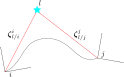
\includegraphics[width=1\columnwidth]{feat_frames}\caption{Vision Factor Geometry}
\label{fig:vision_factor_geometry}
\end{figure}

\begin{align*}
\hat{\zt}_{l/c_{j}}^{c_{j}} & =R_{I}^{c_{j}}\left(\p_{l/I}^{I}-\p_{c_{j}/I}^{I}\right)\\
 & =R_{j}^{c_{j}}R_{I}^{j}\left(\p_{i/I}^{I}+\p_{l/i}^{I}-\left(R_{j}^{I}\p_{c_{j}/j}^{j}+\p_{j/I}^{I}\right)\right)\\
 & =R_{j}^{c_{j}}R_{I}^{j}\left(\p_{i/I}^{I}+R_{i}^{I}\left(R_{c_{i}}^{i}\frac{1}{\rho}\zt_{l/c_{i}}^{c_{i}}+\p_{c_{i}/i}^{i}\right)-\left(R_{j}^{I}\p_{c_{j}/j}^{j}+\p_{j/I}^{I}\right)\right)\\
 & =R_{j}^{c_{j}}R_{I}^{j}\left(\p_{i/I}^{I}+R_{i}^{I}\left(R_{c_{i}}^{i}\frac{1}{\rho}\zt_{l/c_{i}}^{c_{i}}+\p_{c_{i}/i}^{i}\right)\right)-R_{I}^{j}\left(R_{j}^{I}\p_{c_{j}/j}^{j}+\p_{j/I}^{I}\right)\\
 & =R_{j}^{c_{j}}R_{I}^{j}\left(\p_{i/I}^{I}+R_{i}^{I}\left(R_{c_{i}}^{i}\frac{1}{\rho}\zt_{l/c_{i}}^{c_{i}}+\p_{c_{i}/i}^{i}\right)\right)-\left(\p_{c_{j}/j}^{j}+R_{I}^{j}\p_{j/I}^{I}\right)\\
 & =R_{j}^{c_{j}}R_{I}^{j}\left(\p_{i/I}^{I}+R_{i}^{I}\left(R_{c_{i}}^{i}\frac{1}{\rho}\zt_{l/c_{i}}^{c_{i}}+\p_{c_{i}/i}^{i}\right)-\p_{j/I}^{I}\right)-\p_{c_{j}/j}^{j}
\end{align*}
The residual for this measurement is then

\[
r_{\zt}=\mathbb{P}_{\zt}\left(\hat{\zt}_{l/j}^{j}-\bar{\zt}_{l/j}^{j}\right)
\]
where

\[
\mathbb{P}_{\zt}=\begin{bmatrix}\frac{\zt_{i}\times\e_{3}}{\norm{\zt_{i}\times\e_{3}}} & \frac{\zt_{i}\times\zt_{i}\times\e_{3}}{\norm{\zt_{i}\times\zt_{i}\times\e_{3}}}\end{bmatrix}^{\top}
\]


\subsubsection{Jacobians}

The Jacobians of the feature residual are derived below. We will use
the following identities

\begin{align*}
\frac{\partial}{\partial\v}\frac{\v}{\norm{\v}} & =\frac{\frac{\partial}{\partial\v}\v\norm{\v}-\v\frac{\partial}{\partial\v}\norm{\v}}{\v^{\top}\v}\\
 & =\frac{I\norm{\v}-\v\left(\frac{\v}{\norm{\v}}\right)^{\top}}{\v^{\top}\v}
\end{align*}

\begin{align*}
\frac{\partial}{\partial\q}R\left(q\right)\v & =\skew{R\left(\q\right)\v},\quad\frac{\partial}{\partial\q}R\left(q\right)^{\top}\v=-R\left(q\right)^{\top}\skew{\v},\\
\frac{\partial}{\partial\v}\norm{\v} & =\frac{\v^{\top}}{\norm{\v}},\quad\frac{\partial}{\partial a}\frac{1}{a}=-\frac{1}{a^{2}}
\end{align*}

\begin{align*}
\frac{\partial r_{\zeta}}{\partial\p_{i/I}^{I}} & =\frac{\partial r_{\zeta}}{\partial\p_{i/I}^{I}}\mathbb{P}_{\zt}\left(\frac{\hat{\zt}}{\norm{\hat{\zt}}}-\bar{\zt}_{l/j}^{j}\right)\\
 & =\mathbb{P}_{\zt_{i}}\left(\frac{I\norm{\zt_{j}}-\zt_{j}\left(\frac{\zt_{j}}{\norm{\zt_{j}}}\right)^{\top}}{\zt_{j}^{\top}\zt_{j}}\frac{\partial r_{\zeta}}{\partial\p_{i/I}^{I}}\left(R_{j}^{c_{j}}R_{I}^{j}\left(\p_{i/I}^{I}+R_{i}^{I}\left(R_{c_{i}}^{i}\frac{1}{\rho}\zt_{l/c_{i}}^{c_{i}}+\p_{c_{i}/i}^{i}\right)-\left(R_{j}^{I}\p_{c_{j}/j}^{j}+\p_{j/I}^{I}\right)\right)\right)\right)\\
 & =\mathbb{P}_{\zt_{i}}\frac{I\norm{\zt_{j}}-\zt_{j}\left(\frac{\zt_{j}}{\norm{\zt_{j}}}\right)^{\top}}{\zt_{j}^{\top}\zt_{j}}R_{j}^{c_{j}}R_{I}^{j}\\
 & =\mathbb{P}_{\zt_{i}}ZR_{j}^{c_{j}}R_{I}^{j},\quad\quad Z=\frac{I\norm{\zt_{j}}-\zt_{j}\left(\frac{\zt_{j}}{\norm{\zt_{j}}}\right)^{\top}}{\zt_{j}^{\top}\zt_{j}}
\end{align*}

\begin{align*}
\frac{\partial r_{\zeta}}{\partial\q_{I}^{i}} & =\frac{\partial r_{\zeta}}{\partial\q_{I}^{i}}\mathbb{P}_{\zt}\left(\frac{\hat{\zt}}{\norm{\hat{\zt}}}-\bar{\zt}_{l/j}^{j}\right)\\
 & =\mathbb{P}_{\zt}\left(Z\frac{\partial r_{\zeta}}{\partial\q_{I}^{i}}\left(R_{j}^{c_{j}}R_{I}^{j}\left(\p_{i/I}^{I}+R_{i}^{I}\left(R_{c_{i}}^{i}\frac{1}{\rho}\zt_{l/c_{i}}^{c_{i}}+\p_{c_{i}/i}^{i}\right)-\left(R_{j}^{I}\p_{c_{j}/j}^{j}+\p_{j/I}^{I}\right)\right)\right)\right)\\
 & =\mathbb{P}_{\zt}Z\frac{\partial r_{\zeta}}{\partial\q_{i/I}^{I}}\left(R_{j}^{c_{j}}R_{I}^{j}\left(\p_{i/I}^{I}+R_{i}^{I}\left(R_{c_{i}}^{i}\frac{1}{\rho}\zt_{l/c_{i}}^{c_{i}}+\p_{c_{i}/i}^{i}\right)-\left(R_{j}^{I}\p_{c_{j}/j}^{j}+\p_{j/I}^{I}\right)\right)\right)\\
 & =\mathbb{P}_{\zt}ZR_{j}^{c_{j}}R_{I}^{j}\frac{\partial r_{\zeta}}{\partial\q_{I}^{i}}R\left(\q_{I}^{i}\right)^{\top}\left(R_{c_{i}}^{i}\frac{1}{\rho}\zt_{l/c_{i}}^{c_{i}}+\p_{c_{i}/i}^{i}\right)\\
 & =-\mathbb{P}_{\zt}ZR_{j}^{c_{j}}R_{I}^{j}R\left(\q_{I}^{i}\right)^{\top}\skew{R_{c_{i}}^{i}\frac{1}{\rho}\zt_{l/c_{i}}^{c_{i}}+\p_{c_{i}/i}^{i}}
\end{align*}

\begin{align*}
\frac{\partial r_{\zeta}}{\text{\ensuremath{\partial\p_{j/I}^{I}}}} & =\frac{\partial r_{\zeta}}{\partial\p_{j/I}^{I}}\mathbb{P}_{\zt}\left(\frac{\hat{\zt}}{\norm{\hat{\zt}}}-\bar{\zt}_{l/j}^{j}\right)\\
 & =\mathbb{P}_{\zt}Z\frac{\partial r_{\zeta}}{\partial\p_{j/I}^{I}}\left(R_{j}^{c_{j}}R_{I}^{j}\left(\p_{i/I}^{I}+R_{i}^{I}\left(R_{c_{i}}^{i}\frac{1}{\rho}\zt_{l/c_{i}}^{c_{i}}+\p_{c_{i}/i}^{i}\right)-\left(R_{j}^{I}\p_{c_{j}/j}^{j}+\p_{j/I}^{I}\right)\right)\right)\\
 & =\mathbb{P}_{\zt}Z\frac{\partial r_{\zeta}}{\partial\p_{j/I}^{I}}\left(R_{j}^{c_{j}}R_{I}^{j}\left(-\p_{j/I}^{I}\right)\right)\\
 & =-\mathbb{P}_{\zt}ZR_{j}^{c_{j}}R_{I}^{j}
\end{align*}

\begin{align*}
\frac{\partial r_{\zeta}}{\text{\ensuremath{\partial\q_{I}^{j}}}} & =\frac{\partial r_{\zeta}}{\partial\q_{I}^{j}}\mathbb{P}_{\zt}\left(\frac{\hat{\zt}}{\norm{\hat{\zt}}}-\bar{\zt}_{l/j}^{j}\right)\\
 & =\mathbb{P}_{\zt}Z\frac{\partial r_{\zeta}}{\partial\q_{I}^{j}}\left(R_{j}^{c_{j}}R_{I}^{j}\left(\p_{i/I}^{I}+R_{i}^{I}\left(R_{c_{i}}^{i}\frac{1}{\rho}\zt_{l/c_{i}}^{c_{i}}+\p_{c_{i}/i}^{i}\right)-\p_{j/I}^{I}\right)-\p_{c_{j}/j}^{j}\right)\\
 & =\mathbb{P}_{\zt}ZR_{j}^{c_{j}}\left(\frac{\partial r_{\zeta}}{\partial\q_{I}^{j}}R\left(\q_{I}^{j}\right)\left(\p_{i/I}^{I}+R_{i}^{I}\left(R_{c_{i}}^{i}\frac{1}{\rho}\zt_{l/c_{i}}^{c_{i}}+\p_{c_{i}/i}^{i}\right)-\p_{j/I}^{I}\right)-\p_{c_{j}/j}^{j}\right)\\
 & =\mathbb{P}_{\zt}ZR_{j}^{c_{j}}\skew{R\left(\q_{I}^{j}\right)\left(\p_{i/I}^{I}+R_{i}^{I}\left(R_{c_{i}}^{i}\frac{1}{\rho}\zt_{l/c_{i}}^{c_{i}}+\p_{c_{i}/i}^{i}\right)-\p_{j/I}^{I}\right)}
\end{align*}

\begin{align*}
\frac{\partial r_{\zt}}{\partial\rho} & =\frac{\partial r_{\zeta}}{\partial\rho}\mathbb{P}_{\zt}\left(\frac{\hat{\zt}}{\norm{\hat{\zt}}}-\bar{\zt}_{l/j}^{j}\right)\\
 & =\mathbb{P}_{\zt}Z\frac{\partial r_{\zeta}}{\partial\rho}\left(R_{j}^{c_{j}}R_{I}^{j}\left(\p_{i/I}^{I}+R_{i}^{I}\left(R_{c_{i}}^{i}\frac{1}{\rho}\zt_{l/c_{i}}^{c_{i}}+\p_{c_{i}/i}^{i}\right)-\p_{j/I}^{I}\right)-\p_{c_{j}/j}^{j}\right)\\
 & =\mathbb{P}_{\zt}ZR_{j}^{c_{j}}R_{I}^{j}R_{i}^{I}R_{c_{i}}^{i}\frac{\partial r_{\zeta}}{\partial\rho}\frac{1}{\rho}\zt_{l/c_{i}}^{c_{i}}\\
 & =\mathbb{P}_{\zt}ZR_{j}^{c_{j}}R_{I}^{j}R_{i}^{I}R_{c_{i}}^{i}\frac{1}{\rho^{2}}\zt_{l/c_{i}}^{c_{i}}
\end{align*}


\subsection{Keyframe Selection}

New keyframes are selected under two conditions. The first is when
the average parallax exceeds some threshold. The average parallax
between frames $i$ and $j$ of $N$ pixel measurements is given by

\[
\frac{1}{N}\sum_{n=0}^{N-1}\norm{\pi\left(R_{j}^{i}\pi^{-1}\left(\lambda_{n}^{j}\right)-\lambda_{n}^{i}\right)}_{2},
\]
where $\pi$ is the camera projection function which maps pixel measurements
$\lambda^{i}$ into the associated unit vector $\zeta_{i/c}^{c}$
\[
\pi\left(\lambda^{i}\right)=\zeta_{i/c}^{c}
\]
and $R_{j}^{i}$ is the rotation between frames.

We also select keyframes when the number of tracked pixels between
keyframes drops below a specified value.

\subsection{Feature Window Management}

If the feature was originally seen in the last keyframe of the sliding
window, but has been observed in several frames in the window, we
move the anchor to the next keyframe for all the factors corresponding
to that feature. We use our current estimate of the inverse depth
of the feature and our current estimate of the transform between the
two keyframes to initialize the new inverse depth

\begin{align*}
\p_{l/I}^{I}=R_{j}^{I}\p_{l/j}^{j}+\p_{j/I}^{I} & =R_{i}^{I}\p_{l/i}^{i}+\p_{i/I}^{I}\\
R_{j}^{I}\left(R_{c_{j}}^{j}\left(\rho_{j}\zt_{l/c_{j}}^{c_{j}}\right)+\p_{c_{j}/j}^{j}\right)+\p_{j/I}^{I} & =R_{i}^{I}\left(R_{c_{i}}^{i}\left(\rho_{i}\zt_{l/c_{i}}^{c_{i}}\right)+\p_{c_{i}/i}^{i}\right)+\p_{i/I}^{I}\\
\rho_{j}\zt_{l/c_{j}}^{c_{j}} & =R_{j}^{c_{j}}\left(R_{I}^{j}\left(R_{i}^{I}\left(R_{c_{i}}^{i}\left(\rho_{i}\zt_{l/c_{i}}^{c_{i}}\right)+\p_{c_{i}/i}^{i}\right)+\p_{i/I}^{I}-\p_{j/I}^{I}\right)-\p_{c_{j}/j}^{j}\right)\\
\rho_{j} & =\norm{R_{j}^{c_{j}}\left(R_{I}^{j}\left(R_{i}^{I}\left(R_{c_{i}}^{i}\left(\rho_{i}\zt_{l/c_{i}}^{c_{i}}\right)+\p_{c_{i}/i}^{i}\right)+\p_{i/I}^{I}-\p_{j/I}^{I}\right)-\p_{c_{j}/j}^{j}\right)}
\end{align*}

\end{document}
